\documentclass[9pt]{beamer}

\beamertemplatenavigationsymbolsempty
\renewcommand\mathfamilydefault{cmr}

\usepackage{pajmath}
\usepackage{booktabs}
\usepackage{colortbl}

\usepackage{tikz}
\usetikzlibrary{positioning,shapes.misc,calc,backgrounds,scopes} 
\usetikzlibrary{datavisualization}
\usetikzlibrary{datavisualization.formats.functions}
\tikzset{boxed/.style={
  thick,
  draw=black,
  top color=white,
  text height=1.5ex,
  text depth=.25ex
}}


\newcommand\lo{$-1$}
\newcommand\hi{$\phan1$}
\newcommand\ze{$\phan0$}
\newcommand\Ze{$\phan\Vzero$}
\newcommand\pskip{\pause\bigskip}
\newcommand\lspace{\addtolength{\itemsep}{0.5\baselineskip}}

\title{Reinforcement Learning:\\Markov Decision Processes}
\author{BIOE 498/598 PJ}
\date{Spring 2022}

\begin{document}
\frame{\titlepage}

\begin{frame}{Supervised learning vs.\ Reinforcement learning (RL)}

\textbf{Supervised Learning}
\begin{itemize}
	\item Learning from data that has already been collected
	\item Examples: Linear models, Gaussian Process Regression, Neural Networks
\end{itemize}

\pskip
\textbf{Reinforcement Learning}
\begin{itemize}
	\item Learning from trial and error
	\item Examples: Animals, computer chess, self-driving cars
\end{itemize}
	
\end{frame}

\begin{frame}{RL is structured randomness}

\begin{itemize}\lspace
	\item Many RL algorithms rely on random processes to generate data.
	\item RL needs structure to learn from these data.
	\item The most common framework is the \emph{Markov Decision Process} (MDP).
\end{itemize}	

\end{frame}

\begin{frame}{Markov Decision Processes}
	
MDPs describe how an \emph{agent} interacts with its environment.
\bigskip
\begin{itemize}\lspace
	\item At any time, the agent and environment are described by a \textbf{state}.
	\item The agent selects an \textbf{action} to move between states.
	\item Every action and state produce a \textbf{reward}.
	\item The agent's goal is to maximize the total reward it collects.
\end{itemize}

\pskip
MDPs have the \emph{Markov Property}:
\begin{itemize}
	\item All decisions depend only on the current state.
	\item Each state includes all of the relevant history.
\end{itemize}

\end{frame}

\begin{frame}{Markov Decision Processes (continued)}
	
\begin{itemize}\lspace
	\item We denote a state as $s$.
	\item The actions $a\in\mathcal{A}$ available to the agent can depend on the state, so $\mathcal{A} = \mathcal{A}(s)$.
	\item A \textbf{policy} $\pi$ is a function that maps states to actions. The value $\pi(s,a)$ is the probability that the agent will select action $a$ in state $s$.
\end{itemize}
\pskip
\begin{itemize}\lspace
	\item MDPs can be \emph{deterministic} or \emph{stochastic}. 
	\begin{itemize}
		\item Deterministic: Actions always determine the next state.
		\item Stochastic: Actions change the probability that any other state will be the next state.
	\end{itemize}
	\item We will focus on \emph{finite horizon} or \emph{episodic} MDPs.
	\begin{itemize}
		\item Finite horizon MDPs stop (terminate) after a finite number of actions.
		\item A \emph{trajectory} is a single pass through a finite horizon MDP.
	\end{itemize}
\end{itemize}

\end{frame}

\begin{frame}{Gridworld}

Imagine a simple maze on a $4\times 4$ grid.
\begin{itemize}
	\item Each square is a state.
	\item The walls determine the available actions at each state.
	\item The agent starts in the bottom left and must reach the top right.
	\item The objective is to finish the maze in as few steps as possible.
\end{itemize}

\begin{center}
	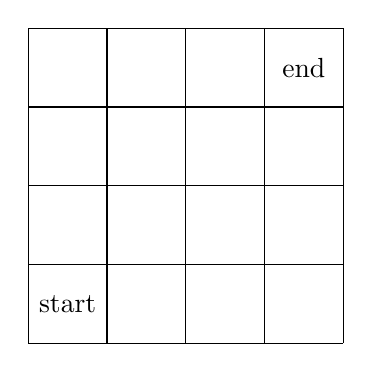
\begin{tikzpicture}
		\draw (0,0) grid (4,4);
		\node at (0.5,0.5) {start};
		\node at (3.5,3.5) {end};
	\end{tikzpicture}
\end{center}

\end{frame}

\begin{frame}{A Monte Carlo approach}

\begin{columns}
\begin{column}{0.5\textwidth}
	\begin{itemize}
		\item Each grid square is a state.
		\item Actions: move up, down, left, or right, but the agent cannot leave the grid.
		\item Reward: $-1$ for each step.
		\item Policy: Random.
	\end{itemize}
	
\bigskip
Starting from a random state, make random moves until the agent reaches the end.

\bigskip
Repeat may times and average the total rewards from each trajectory.
\end{column}

\begin{column}{0.5\textwidth}
	\begin{center}
		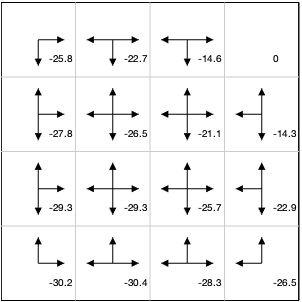
\includegraphics[width=\textwidth]{figures/gridworld1a.png}	
	\end{center}
\end{column}

\end{columns}

\end{frame}

\begin{frame}{From randomness to a better policy (policy improvement)}
\begin{columns}

\begin{column}{0.5\textwidth}
	\begin{center}
		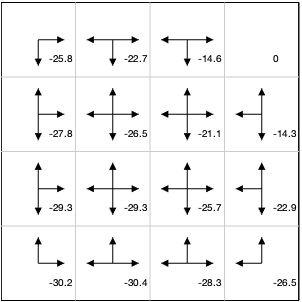
\includegraphics[width=\textwidth]{figures/gridworld1a.png}	
	\end{center}
\end{column}

\begin{column}{0.5\textwidth}
	\begin{center}
		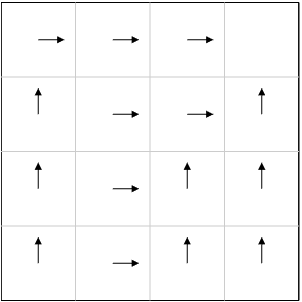
\includegraphics[width=\textwidth]{figures/gridworld1b.png}	
	\end{center}
\end{column}

\end{columns}
\end{frame}

\begin{frame}
\begin{columns}
\begin{column}{0.3\textwidth}
	Let's add an internal wall for the agent to navigate.
	\begin{center}
		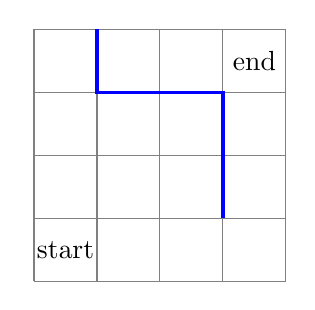
\begin{tikzpicture}[scale=0.8]
			\draw [color=gray,thin] (0,0) grid (4,4);
			\node at (0.5,0.5) {start};
			\node at (3.5,3.5) {end};
			\draw [very thick,blue] (1,4) -- (1,3) -| (3,1);
		\end{tikzpicture}
	\end{center}
\end{column}

\begin{column}{0.7\textwidth}
	\begin{center}
		\pause
		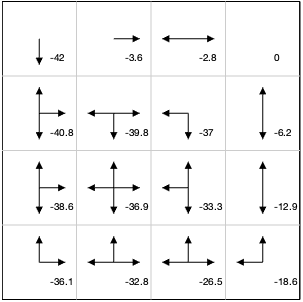
\includegraphics[width=0.6\textwidth]{figures/gridworld2a.png}
		\pause	
		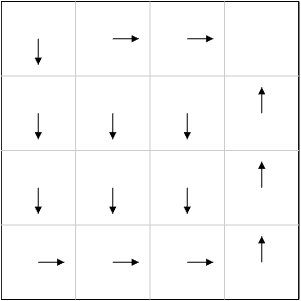
\includegraphics[width=0.6\textwidth]{figures/gridworld2b.png}	
	\end{center}
\end{column}
\end{columns}
\end{frame}

\begin{frame}
\begin{columns}
\begin{column}{0.3\textwidth}
	Can the agent learn a shortcut?
	\begin{center}
		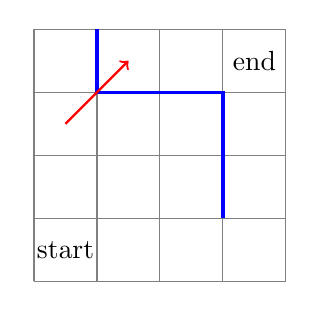
\begin{tikzpicture}[scale=0.8]
			\draw [thin,gray] (0,0) grid (4,4);
			\node at (0.5,0.5) {start};
			\node at (3.5,3.5) {end};
			\draw [very thick,blue] (1,4) -- (1,3) -| (3,1);
			\draw [thick,red,->] (0.5,2.5) -- (1.5,3.5);
		\end{tikzpicture}
	\end{center}
\end{column}

\begin{column}{0.7\textwidth}
	\begin{center}
		\pause
		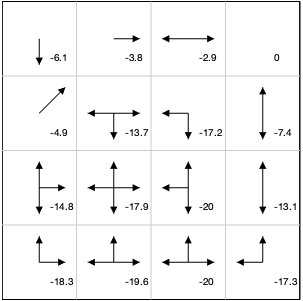
\includegraphics[width=0.6\textwidth]{figures/gridworld3a.png}
		\pause	
		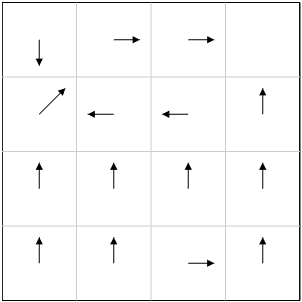
\includegraphics[width=0.6\textwidth]{figures/gridworld3b.png}	
	\end{center}
\end{column}
\end{columns}
\end{frame}

\begin{frame}{Summary}

\begin{itemize}\lspace
	\item RL agents can learn by trial and error.
	\item MDPs provide a mathematical structure for RL problems.
	\item The choice of states, actions, and rewards is critical.
	\item<2-> \textbf{Next time:} What are we learning from our random maze walks?
\end{itemize}

\end{frame}

\end{document}
